\documentclass[tikz]{standalone}
\usepackage{pgfplots}
\pgfplotsset{width = 10cm,compat = 1.15}
\usepgfplotslibrary{fillbetween}
\usepgfplotslibrary{dateplot}
\usetikzlibrary{angles, quotes}
\selectcolormodel{gray}
\usepackage{physics}
\usepackage{amsfonts}

\begin{document}

\pgfmathdeclarefunction{gauss}{3}{%
  \pgfmathparse{1/(#3*sqrt(2*pi))*exp(-((#1-#2)^2)/(2*#3^2))}%
}

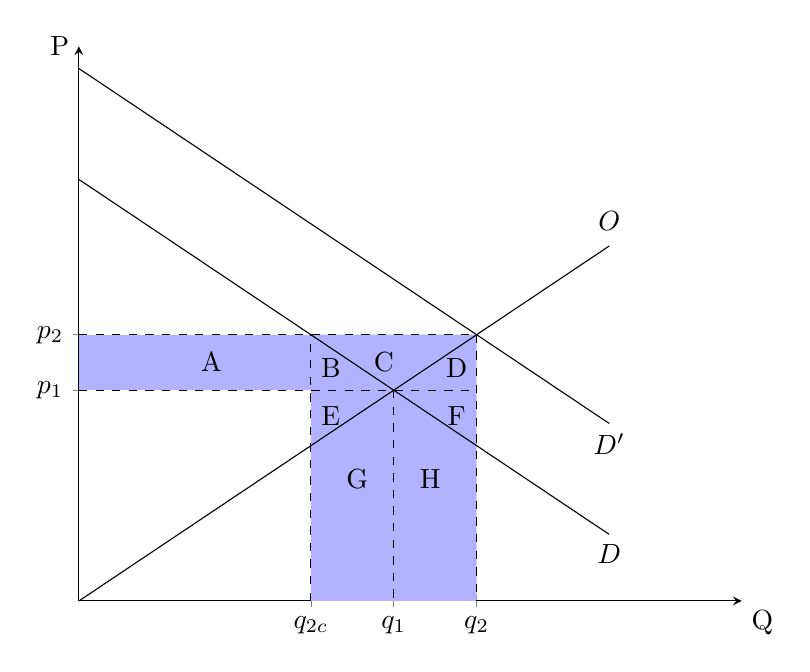
\begin{tikzpicture}
\begin{axis}[
    ylabel = {P},
    xlabel = {Q},
    axis x line = center,
    axis y line = center,
    xlabel style={align = center, below right},
    ylabel style={align = left, left},
    xmin=0,xmax=5,
    ymin = 0, ymax = 5,
    xtick={1.75,19/8,3}, xticklabels = {$q_{2c}$, $q_{1}$, $q_{2}$},
    ytick={1.9, 2.4}, yticklabels = {$p_{1}$, $p_{2}$},
    clip=false,
]

\addplot [domain = 0:4, smooth, samples = 400, name path = A] {0.8*x};
\addplot [domain = 0:4, smooth, samples = 400, name path = B] {3.8-0.8*x};
\addplot [domain = 0:4, smooth, samples = 400, name path = C] {4.8-0.8*x};
\draw [dashed, name path = D] (0,1.9) -- (3,1.9);
\draw [dashed, name path = E] (19/8,1.9) -- (19/8,0);
\draw [dashed, name path = F] (0,2.4) -- (3,2.4);
\draw [dashed, name path = G] (3,2.4) -- (3,0);
\draw [dashed, name path = H] (1.75,0) -- (1.75,2.4);
\path [name path=xaxis]
		(\pgfkeysvalueof{/pgfplots/xmin},0) --
		(\pgfkeysvalueof{/pgfplots/xmax},0);
\node[below] at (axis cs:4,3.6){$O$};
\node[below] at (axis cs:4,0.6){$D$};
\node[below] at (axis cs:4,1.6){$D'$};
\addplot[blue!30] fill between[of=D and F, soft clip={domain = 0:1.75}];
\addplot[blue!30] fill between[of=B and D, soft clip={domain = 1.75:19/8}];
\addplot[blue!30] fill between[of=B and F, soft clip={domain = 1.75:19/8}];
\addplot[blue!30] fill between[of=A and F, soft clip={domain = 19/8:3}];
\addplot[blue!30] fill between[of=A and D, soft clip={domain = 19/8:3}];
\addplot[blue!30] fill between[of=D and xaxis, soft clip={domain = 1.75:3}];


\node[] at (axis cs:1,2.15){A};
\node[] at (axis cs:1.9,2.1){B};
\node[] at (axis cs:2.3,2.15){C};
\node[] at (axis cs:2.85,2.1){D};
\node[] at (axis cs:1.9,1.67){E};
\node[] at (axis cs:2.85,1.67){F};
\node[] at (axis cs:2.1,1.1){G};
\node[] at (axis cs:2.65,1.1){H};

\end{axis}
\end{tikzpicture}

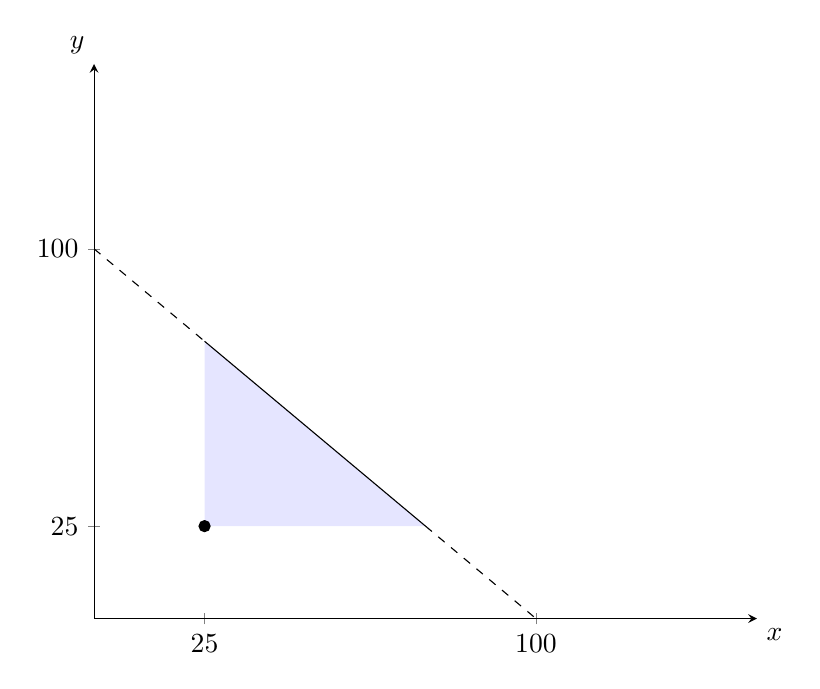
\begin{tikzpicture}
\begin{axis}[
    xlabel = {$x$},
    ylabel = {$y$},
    axis x line = center,
    axis y line = center,
    xlabel style={below right},
    ylabel style={above left},
    xmin=0,xmax=150,
    ymin=0, ymax=150,
    xtick={25,100},
    ytick={25,100},
    %xticklabels={auto},
    %yticklabels={$w^*$},
    restrict y to domain=-200:200
]

\addplot [domain = 0:25,smooth,name path = A, dashed] {100-x};
\addplot [domain = 75:100,smooth,name path = A, dashed] {100-x};
\addplot [domain = 25:75,smooth,name path = A] {100-x};
% %\addlegendentry{Rmg}
% %\addlegendentry{Cmg Formal}
% %\addlegendentry{Cmg Informal}
\addplot[mark=*] coordinates {(25,25)};
\path [name path = B] (25,75) |- (75,25);

\addplot[blue!10] fill between[of=A and B];
\end{axis}
\end{tikzpicture}

\begin{tikzpicture}
\begin{axis}[
    xlabel = {$x$},
    ylabel = {$y$},
    axis x line = center,
    axis y line = center,
    xlabel style={below right},
    ylabel style={above left},
    xmin=0,xmax=150,
    ymin=0, ymax=150,
    xtick={100},
    ytick={100},
    %xticklabels={auto},
    %yticklabels={$w^*$},
    restrict y to domain=-200:200
]

\addplot [domain = 0:100,smooth,name path = A, dashed] {50-x};
\addplot [domain = 0:100,smooth,name path = A] {100-x};

\end{axis}
\end{tikzpicture}

\begin{tikzpicture}
  \draw [|->](0,0)--(4.5,0);
  \draw (0,-.1)--(0,.1);
  \draw (4,-.2)--(4,.2);
  \node[align=left,below] at (0.2,-0.1) {0};
  \node[align=left,below] at (4.2,-0.1) {1};
  \draw [|->](0,0)--(0,-1);
  \draw [|->](4,0)--(4,1.2);
  \node[align=left,below] at (0,-1) {R\$50 milhões};
  \node[align=left,above] at (4,1.2) {R\$60 milhões};
\end{tikzpicture}

\begin{tikzpicture}
\begin{axis}[
    xlabel = {$r$},
    ylabel={VPL(1.000 Reais)},
    axis x line = center,
    axis y line = center,
    xlabel style={below right},
    ylabel style={above left},
    xmin=0,xmax=0.2,
    xtick={0.02,0.06,0.1,0.14,0.18},
]

\addplot [domain = 0.02:0.2,smooth,name path = A, samples = 400] {10/(x*(1+x)^2)*(1-(1/(1+x))^13)-2/x*(1-(1/(1+x))^15)-50};
\draw [|->, dashed](0.082,-10)--(0.082,0);
\node[] at (axis cs:0.082,-11){TIR = 8,2\%};
% %\addlegendentry{Rmg}
% %\addlegendentry{Cmg Formal}
% %\addlegendentry{Cmg Informal}
%\draw[->] (2.5,3.4) -- (1.55,2.05) ;
%\node[] at (axis cs:3.2,3.4){Dotação Inicial};

\end{axis}
\end{tikzpicture}

\begin{tikzpicture}
\begin{axis}[
    xlabel = {$C_1$},
    ylabel={$C_2$},
    axis x line = center,
    axis y line = center,
    xlabel style={below right},
    ylabel style={above left},
    xmin=0,xmax=5,
    ymin = 0, ymax = 6,
    xtick={3.25, 4.5}, xticklabels = {$C_1^*$, $T$},
    ytick={2.25, 5}, yticklabels = {$C_2^*$, $S$},
]

\addplot [domain = 0:4.6, smooth,name path = A, samples = 400] {-0.2*x^2-0.2*x+5};
\addplot [domain = 2.5:4.5, smooth, samples = 400] {(35/(x^(0.7))^(1/0.3)};
\addplot [domain = 2.2:4.5, smooth, samples = 400] {(25/(x^(0.7))^(1/0.3)};
\addplot[mark=*] coordinates {(3.25,2.25)};
\addplot[mark=*] coordinates {(4.02,0.98)};
\draw [dashed] (3.25,0) -- (3.25,2.25);
\draw [dashed] (0,2.25) -- (3.25,2.25);
\node[] at (axis cs:2.8,4.2){$CIS_1$};
\node[] at (axis cs:2.05,3.4){$CIS_2$};
\node[above] at (axis cs:3.35,2.25){$X$};
\node[below] at (axis cs:3.9,0.98){$W$};
% %\addlegendentry{Rmg}
% %\addlegendentry{Cmg Formal}
% %\addlegendentry{Cmg Informal}
%\draw[->] (2.5,3.4) -- (1.55,2.05) ;
%\node[] at (axis cs:3.2,3.4){Dotação Inicial};

\end{axis}
\end{tikzpicture}

\begin{tikzpicture}
\begin{axis}[
    ylabel = {Juros},
    xlabel = {Investimento,\\ Poupança},
    axis x line = center,
    axis y line = center,
    xlabel style={align = left, below right},
    ylabel style={align = left, left},
    xmin=0,xmax=5,
    ymin = 0, ymax = 5,
    xtick={125/72,35/18,38/18}, xticklabels = { , , },
    ytick={35/18, 53/18, 56/18, 71/18}, yticklabels = {$TJC$, $i$, $i'$, $ROI$},
    clip=false,
]

\addplot [dashed, domain = 1:4, smooth, samples = 400] {x};
\addplot [domain = 1:4, smooth, samples = 400] {1+x};
\addplot [dashed, domain = 1:4, smooth, samples = 400] {5.5-0.8*x};
\addplot [domain = 1:4, smooth, samples = 400] {4.5-0.8*x};
\addplot [domain = 1:4, smooth, samples = 400] {4.8-0.8*x};
\draw [dashed] (125/72,0) -- (125/72,56/18);
\draw [dashed] (35/18,0) -- (35/18,71/18);
\draw [dashed] (38/18,0) -- (38/18,56/18);
\draw [dashed] (0,35/18) -- (35/18,35/18);
\draw [dashed] (0,53/18) -- (35/18,53/18);
\draw [dashed] (0,56/18) -- (38/18,56/18);
\draw [dashed] (0,71/18) -- (35/18,71/18);
\draw [dashed, |-|] (125/72,-0.2) -- (35/18,-0.2);
\draw [dashed, |-|] (35/18,-0.2) -- (38/18,-0.2);
\node[] at (axis cs:4,4.2){$O_0$};
\node[left] at (axis cs:1.1,2.15){$O_t$};
\node[] at (axis cs:4,2.1){$D_0$};
\node[left] at (axis cs:1.1,3.6){$D_t$};
\node[left] at (axis cs:1.1,4.2){$D'_t$};
\node[below] at (axis cs:265/144,-0.2){\tiny $\Delta I$};
\node[below] at (axis cs:73/36,-0.2){\tiny $\Delta C$};
% %\addlegendentry{Rmg}
% %\addlegendentry{Cmg Formal}
% %\addlegendentry{Cmg Informal}
%\draw[->] (2.5,3.4) -- (1.55,2.05) ;
%\node[] at (axis cs:3.2,3.4){Dotação Inicial};

\end{axis}
\end{tikzpicture}

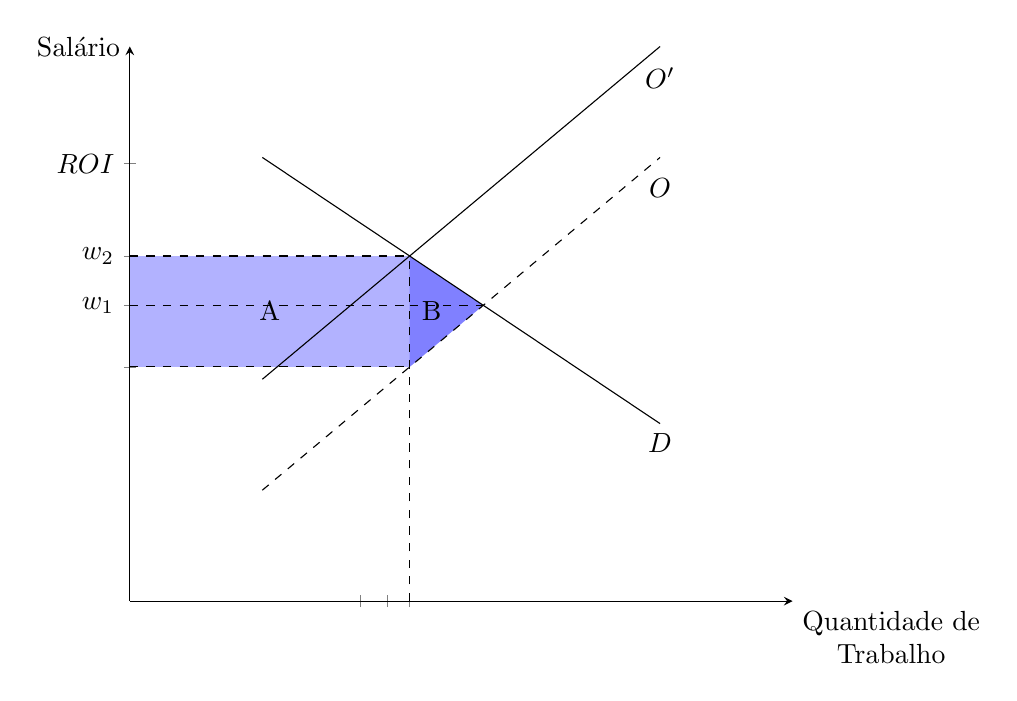
\begin{tikzpicture}
\begin{axis}[
    ylabel = {Salário},
    xlabel = {Quantidade de\\Trabalho},
    axis x line = center,
    axis y line = center,
    xlabel style={align = center, below right},
    ylabel style={align = left, left},
    xmin=0,xmax=5,
    ymin = 0, ymax = 5,
    xtick={125/72,35/18,38/18}, xticklabels = { , , },
    ytick={38/18, 48/18, 56/18, 71/18}, yticklabels = {, $w_{1}$, $w_{2}$, $ROI$},
    clip=false,
]

\addplot [dashed, domain = 1:4, smooth, samples = 400, name path = A] {x};
\addplot [domain = 1:4, smooth, samples = 400, name path = B] {1+x};
\addplot [domain = 1:4, smooth, samples = 400, name path = C] {4.8-0.8*x};
\draw [dashed, name path = D] (38/18,0) -- (38/18,56/18);
\draw [dashed, name path = E] (0,38/18) -- (38/18,38/18);
\draw [dashed, name path = F] (0,48/18) -- (38/18,48/18);
\draw [dashed, name path = G] (38/18,48/18) -- (48/18,48/18);
\draw [dashed, name path = H] (0,56/18) -- (38/18,56/18);
\node[below] at (axis cs:4,3.9){$O$};
\node[below] at (axis cs:4,4.9){$O'$};
\node[below] at (axis cs:4,1.6){$D$};
\addplot[blue!30] fill between[of=E and H];
\addplot[blue!50] fill between[of=A and C, soft clip={domain = 38/18:48/18}];
\node[] at (axis cs:19/18,47/18){A};
\node[] at (axis cs:41/18,47/18){B};
\end{axis}
\end{tikzpicture}

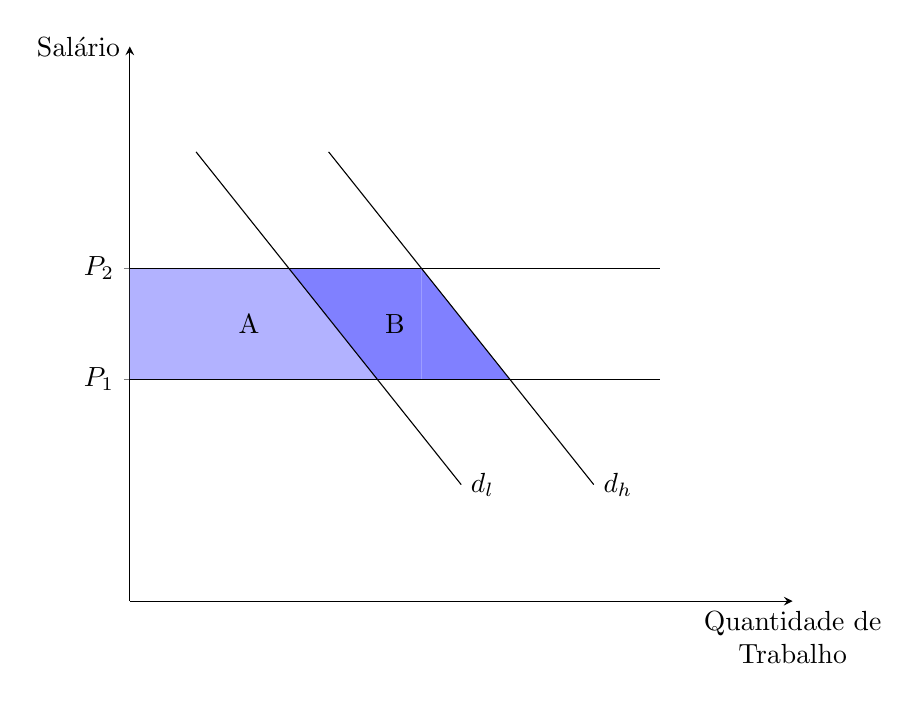
\begin{tikzpicture}
\begin{axis}[
    ylabel = {Salário},
    xlabel = {Quantidade de\\Trabalho},
    axis x line = center,
    axis y line = center,
    xlabel style={align = center, below},
    ylabel style={align = center, left},
    xmin=0,xmax=5,
    ymin = 0, ymax = 5,
    xtick={0}, xticklabels = {},
    ytick={2, 3}, yticklabels = {$P_{1}$, $P_{2}$},
    clip=false,
]

\addplot [domain = 0:4, smooth, samples = 400, name path = A] {2};
\addplot [domain = 0:4, smooth, samples = 400, name path = B] {3};
\addplot [domain = 0.5:2.5, smooth, samples = 400, name path = C] {4.8-1.5*x};
\addplot [domain = 1.5:3.5, smooth, samples = 400, name path = D] {6.3-1.5*x};
\node[right] at (axis cs:2.5,1.05){$d_l$};
\node[right] at (axis cs:3.5,1.05){$d_h$};
\addplot[blue!30] fill between[of=A and B, soft clip={domain = 0:18/15}];
\addplot[blue!30] fill between[of=A and C, soft clip={domain = 18/15:28/15}];
\addplot[blue!50] fill between[of=C and B, soft clip={domain = 18/15:28/15}];
\addplot[blue!50] fill between[of=A and B, soft clip={domain = 28/15:33/15}];
\addplot[blue!50] fill between[of=A and D, soft clip={domain = 33/15:43/15}];
\node[] at (axis cs:0.9,2.5){A};
\node[] at (axis cs:2,2.5){B};
\end{axis}
\end{tikzpicture}

\end{document}
